\documentclass[11pt,letterpaper]{article}
\usepackage[margin=0.62in,top=0.69in,bottom=0.66in,headheight=15pt,headsep=13pt,footskip=24pt]{geometry}
\usepackage{tikz,amsmath,amssymb,fancyhdr,array}
\usetikzlibrary{arrows.meta}
\usepackage[T1]{fontenc}\usepackage{lmodern}
\renewcommand{\familydefault}{\sfdefault}
\pagestyle{fancy}\fancyhf{}\fancyhead[L]{\small Week 71 / Can you hear the room? / Grades 4--5}
\fancyfoot[L]{\scriptsize Bellingham Math Circle / Week 71 / GGT71-S-v1}\fancyfoot[R]{\scriptsize\thepage}
\renewcommand{\headrulewidth}{0.4pt}\renewcommand{\footrulewidth}{0pt}
\setlength{\parindent}{0pt}\setlength{\parskip}{8pt}
\newcommand{\problem}[2]{\textbf{Problem #1:} #2\par}

\newcommand{\squareABA}{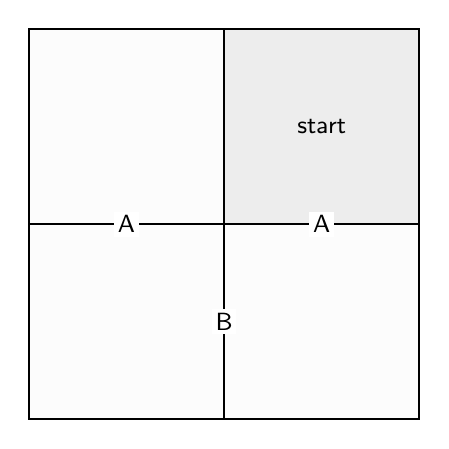
\begin{tikzpicture}[scale=0.62]
\fill[gray!14] (0.00000000,0.00000000)--(4.00000000,0.00000000)--(4.00000000,4.00000000)--(0.00000000,4.00000000)--cycle;
\fill[gray!2] (0.00000000,0.00000000)--(4.00000000,0.00000000)--(4.00000000,-4.00000000)--(0.00000000,-4.00000000)--cycle;
\fill[gray!2] (0.00000000,0.00000000)--(-4.00000000,0.00000000)--(-4.00000000,-4.00000000)--(0.00000000,-4.00000000)--cycle;
\fill[gray!2] (0.00000000,0.00000000)--(-4.00000000,0.00000000)--(-4.00000000,4.00000000)--(0.00000000,4.00000000)--cycle;
\draw[thick] (0.00000000,0.00000000)--(4.00000000,0.00000000)--(4.00000000,4.00000000)--(0.00000000,4.00000000)--cycle;
\draw[thick] (0.00000000,0.00000000)--(4.00000000,0.00000000)--(4.00000000,-4.00000000)--(0.00000000,-4.00000000)--cycle;
\draw[thick] (0.00000000,0.00000000)--(-4.00000000,0.00000000)--(-4.00000000,-4.00000000)--(0.00000000,-4.00000000)--cycle;
\draw[thick] (0.00000000,0.00000000)--(-4.00000000,0.00000000)--(-4.00000000,4.00000000)--(0.00000000,4.00000000)--cycle;
\node[fill=white,inner sep=1.4pt,font=\small]at(2.00000000,0.00000000){A};
\node[fill=white,inner sep=1.4pt,font=\small]at(0.00000000,-2.00000000){B};
\node[fill=white,inner sep=1.4pt,font=\small]at(-2.00000000,0.00000000){A};
\node[font=\small]at(2.00000000,2.00000000){start};
\end{tikzpicture}}
\newcommand{\rhombusABA}{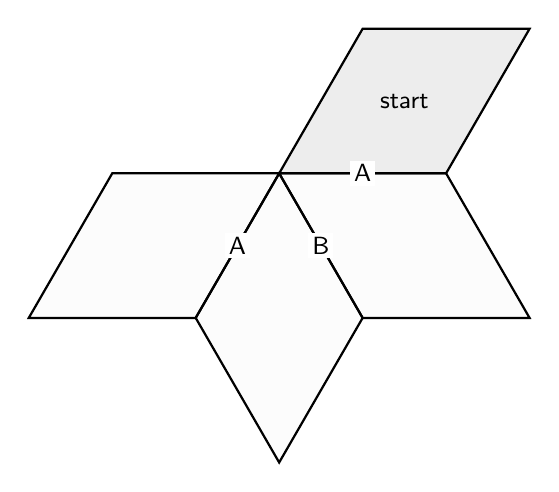
\begin{tikzpicture}[scale=0.53]
\fill[gray!14] (0.00000000,0.00000000)--(4.00000000,0.00000000)--(6.00000000,3.46410162)--(2.00000000,3.46410162)--cycle;
\fill[gray!2] (0.00000000,0.00000000)--(4.00000000,0.00000000)--(6.00000000,-3.46410162)--(2.00000000,-3.46410162)--cycle;
\fill[gray!2] (0.00000000,0.00000000)--(-2.00000000,-3.46410162)--(0.00000000,-6.92820323)--(2.00000000,-3.46410162)--cycle;
\fill[gray!2] (0.00000000,0.00000000)--(-2.00000000,-3.46410162)--(-6.00000000,-3.46410162)--(-4.00000000,-0.00000000)--cycle;
\draw[thick] (0.00000000,0.00000000)--(4.00000000,0.00000000)--(6.00000000,3.46410162)--(2.00000000,3.46410162)--cycle;
\draw[thick] (0.00000000,0.00000000)--(4.00000000,0.00000000)--(6.00000000,-3.46410162)--(2.00000000,-3.46410162)--cycle;
\draw[thick] (0.00000000,0.00000000)--(-2.00000000,-3.46410162)--(0.00000000,-6.92820323)--(2.00000000,-3.46410162)--cycle;
\draw[thick] (0.00000000,0.00000000)--(-2.00000000,-3.46410162)--(-6.00000000,-3.46410162)--(-4.00000000,-0.00000000)--cycle;
\node[fill=white,inner sep=1.4pt,font=\small]at(2.00000000,0.00000000){A};
\node[fill=white,inner sep=1.4pt,font=\small]at(1.00000000,-1.73205081){B};
\node[fill=white,inner sep=1.4pt,font=\small]at(-1.00000000,-1.73205081){A};
\node[font=\small]at(3.00000000,1.73205081){start};
\end{tikzpicture}}

\newcommand{\lines}[1]{\foreach\n in{1,...,#1}{\noindent\rule{\linewidth}{.2pt}\par\vspace{.22in}}}
\newcommand{\rectroom}[3]{\begin{tikzpicture}[scale=#3]
\draw[thick](0,0)rectangle(#1,#2);
\node[below]at({#1/2},0){A};\node[left]at(0,{#2/2}){B};\node[above]at({#1/2},#2){C};\node[right]at(#1,{#2/2}){D};
\end{tikzpicture}}
\newcommand{\rhombusroom}[1]{\begin{tikzpicture}[scale=#1]
\draw[thick](0,0)--(4,0)--(6,3.46410162)--(2,3.46410162)--cycle;
\node[below]at(2,0){A};\node[above left]at(1,1.73205081){B};\node[above]at(4,3.46410162){C};\node[below right]at(5,1.73205081){D};
\draw(.65,0)arc(0:60:.65);\node[font=\scriptsize]at(.92,.34){$60^\circ$};
\end{tikzpicture}}
\newcommand{\tilewindow}[4]{% integer minimum, max, xscale, start marker
\begin{tikzpicture}[x=#3cm,y=1cm]
\foreach\i in{#1,...,#2}{\draw[gray!65](2*\i,2*#1)--(2*\i,2*#2);\draw[gray!65](2*#1,2*\i)--(2*#2,2*\i);}
\pgfmathtruncatemacro{\last}{#2-1}
\foreach\i in{#1,...,#2}{\foreach\j in{#1,...,\last}{
\pgfmathtruncatemacro{\parity}{mod(abs(\i),2)}
\ifnum\parity=0
\node[fill=white,inner sep=.5pt,font=\scriptsize]at(2*\i,2*\j+1){B};
\node[fill=white,inner sep=.5pt,font=\scriptsize]at(2*\j+1,2*\i){A};
\else
\node[fill=white,inner sep=.5pt,font=\scriptsize]at(2*\i,2*\j+1){D};
\node[fill=white,inner sep=.5pt,font=\scriptsize]at(2*\j+1,2*\i){C};
\fi}}
\draw[very thick](0,0)rectangle(2,2);
\ifnum#4=1\fill(1,1)circle(2pt);\fi
\end{tikzpicture}}
\begin{document}
A shot starts inside the room and bounces off its walls. Record the wall letters in the order hit. Stop after the last letter you want to record. A shot that hits a corner is not allowed.

One partner draws a shot with a ruler; the other checks it. To check a bounce, reflect the next room across the wall. The shot continues in a straight line through the reflected copy. Swap jobs for the next shot.

\begin{center}
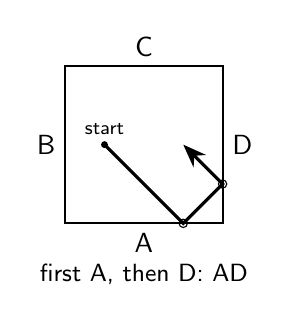
\begin{tikzpicture}[scale=.50]
\draw[thick](0,0)rectangle(4,4);
\node[below]at(2,0){A};\node[left]at(0,2){B};\node[above]at(2,4){C};\node[right]at(4,2){D};
\fill(1,2)circle(2.5pt);\node[above,font=\scriptsize]at(1,2){start};
\draw[very thick,-{Stealth}](1,2)--(3,0)--(4,1)--(3,2);
\draw(3,0)circle(3pt);\draw(4,1)circle(3pt);
\node[below,font=\small]at(2,-.8){first A, then D: AD};
\end{tikzpicture}\hspace{.65in}
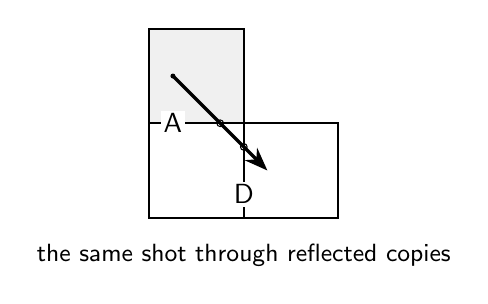
\begin{tikzpicture}[scale=.30]
\fill[gray!12](0,0)rectangle(4,4);
\draw[thick](0,0)rectangle(4,4);\draw[thick](0,0)rectangle(4,-4);\draw[thick](4,0)rectangle(8,-4);
\node[fill=white,inner sep=1pt]at(1,0){A};\node[fill=white,inner sep=1pt]at(4,-3){D};
\fill(1,2)circle(3pt);\draw[very thick,-{Stealth}](1,2)--(5,-2);
\draw(3,0)circle(4pt);\draw(4,-1)circle(4pt);
\node[below,font=\small]at(4,-4.7){the same shot through reflected copies};
\end{tikzpicture}
\end{center}
\problem{1}{Find six different three-letter bounce words in the square. Draw straight shots from the dot through the reflected copies. Write each word by the end of its shot. Your partner checks the crossed walls and any corner hits.}
\begin{center}\tilewindow{-2}{3}{1}{1}\end{center}
\newpage
\problem{2}{Can a shot begin ABA in each room? Start anywhere inside the shaded room. Try to cross A, then B, then A with one straight line, without leaving the drawn copies. Draw a shot wherever it works. Explain any impossibility.}
\vspace{.12in}
\begin{center}
\begin{tabular}{c@{\hspace{.35in}}c}
\squareABA&\rhombusABA\\[7pt]
square copies&$60^\circ$ rhombus copies
\end{tabular}
\end{center}
\vspace{.10in}
Copy a successful shot into its single room. Use a mirror on each wall to check that the incoming line and the reflection of the outgoing line line up.
\begin{center}
\rectroom{4}{4}{.85}\hspace{.70in}\rhombusroom{.80}
\end{center}
\vspace{.18in}\lines{3}
\newpage
\problem{3}{One partner secretly chooses a room and draws a checked shot with at least three bounces. Give only its word. The other partner circles the rooms they have not ruled out. To rule out a room, explain why the word is impossible there. Then reveal the shot and swap jobs.}
You may reuse a checked shot from Problems 1--2. For new shots, use the square and rectangle windows on page 4, or the mirror and large rhombus rooms on page 5. Keep your drawing hidden until the guess.

Failing to find a shot is not a reason to rule out a room.
\begin{center}
\begin{tabular}{c@{\hspace{.50in}}c}
\rectroom{4}{4}{.80}&\rectroom{8}{4}{.80}\\[5pt]
square&wide rectangle
\end{tabular}\par\vspace{.16in}
\rhombusroom{1.05}\par
$60^\circ$ rhombus
\end{center}
\vspace{.14in}
\begin{tabular}{@{}p{2.5in}p{4.2in}@{}}
word & rooms not ruled out\\[12pt]
\hrulefill & square\qquad wide rectangle\qquad rhombus\\[30pt]
\hrulefill & square\qquad wide rectangle\qquad rhombus\\[30pt]
\hrulefill & square\qquad wide rectangle\qquad rhombus
\end{tabular}
\newpage
\problem{4}{Draw three shots starting inside the bold square, with different words of at least three bounces. Each shot must hit both a horizontal and a vertical wall. Move each shot to the wide rectangle without changing its bounce word. Could any bounce word tell these two rooms apart? Explain why, or find a word that only one room can make.}
\begin{center}
\tilewindow{-1}{2}{1}{0}\par\vspace{.22in}
\tilewindow{-1}{2}{2}{0}
\end{center}
\vspace{.14in}\lines{3}
\newpage
Extra workspace for Problems 2--3. Draw new rhombus shots here. Stand the mirror on each wall hit: the incoming line and the mirror image of the outgoing line must line up. Keep the checked drawing to reveal after the guess.
\begin{center}
\rhombusroom{1.90}\par\vspace{.1in}
word: \rule{2.8in}{.3pt}\par\vspace{.45in}
\rhombusroom{1.90}\par\vspace{.1in}
word: \rule{2.8in}{.3pt}
\end{center}
\end{document}
